%%%%%%%%%%%%%%%%%%%%%%%%%%%%%%%%%%%%%%%%%%%%%%%%%%%%%%%%%%%%%%%%%
%%% %
%%% % weiiszablon.tex
%%% % The Faculty of Electrical and Computer Engineering
%%% % Rzeszow University Of Technology diploma thesis Template
%%% % Szablon pracy dyplomowej Wydziału Elektrotechniki 
%%% % i Informatyki PRz
%%% % January, 2024
%%%%%%%%%%%%%%%%%%%%%%%%%%%%%%%%%%%%%%%%%%%%%%%%%%%%%%%%%%%%%%%%%

\documentclass[12pt,twoside]{article}

\usepackage{weiiszablon}

\author{Imię Nazwisko}

% np. EF-123456, EN-654321, ...
\studentID{XX-??????}

\title{Temat pracy}
\titleEN{Temat pracy po angielsku}


%%% wybierz rodzaj pracy wpisując jeden z poniższych numerów: ...
% 1 = inżynierska	% BSc
% 2 = magisterska	% MSc
% 3 = doktorska		% PhD
% 4 = praca inżynierska
%%% na miejsce zera w linijce poniżej
\newcommand{\rodzajPracyNo}{0}


%%% promotor
\supervisor{(tytuł naukowy przed) Imię i nazwisko opiekuna (stanowisko po)}
%% przykład: dr hab. inż. Józef Nowak, prof. PRz

%%% promotor ze stopniami naukowymi po angielsku
\supervisorEN{Prof. Imię i nazwisko opiekuna, (academic degree)}

\abstract{Treść streszczenia po polsku}
\abstractEN{Treść streszczenia po angielsku}

\keywords{max. 5 słów kluczowych w 2 wierszach, oddzielanych przecinkami}
\keywordsEN{max. five keywords in English}


\begin{document}

% strona tytułowa
\maketitle

\blankpage

% spis treści
\tableofcontents

\clearpage
\blankpage


\section*{Wykaz symboli, oznaczeń i skrótów (opcjonalny)}
\addcontentsline{toc}{section}{Wykaz symboli, oznaczeń i skrótów (opcjonalny)}%

1 $\div$ 2 stron wykaz ważniejszych symboli i oznaczeń (jeśli jest potrzebny).

\section{Wstęp/wprowadzenie}
1 $\div$ 5 stron charakterystyka problematyki w świetle aktualnego stanu wiedzy i~techniki, ze wskazaniem na zagadnienia istotne z punktu widzenia realizowanej pracy.
Na trzeciej stronie można zamieścić podziękowania dla osób, które przyczyniły się do powstania pracy dyplomowej.
Na kolejnej stronie nieparzystej rozpoczyna się spis treści.
Po spisie treści zalecane jest umieszczenie wykazu użytych symboli, oznaczeń i~akronimów.
Od tego miejsca rozpoczyna się numeracja rozdziałów.
Na następnej stronie umieszcza się wprowadzenie do pracy (scharakteryzowanie problematyki pracy, uzasadnienie wyboru tematyki) oraz przedstawia: cel i/lub tezę pracy, zakres pracy, przyjęte założenia itp.
Ostatni akapit wstępu musi zawierać zwięzłe sformułowanie celu i zakresu pracy. 
\\
\textcolor{red}{
Uwaga: \\
Jeżeli decydujesz się wykorzystywać \LaTeX'a, ignoruj ogólny dokument dotyczący formatowania pracy dyplomowej na WEiI -- jest przeznaczony dla użytkowników innych edytorów tekstu. Korzystaj z załączonego arkusza stylu, stosuj formatowanie znaczeniowe (nie wymuszaj formatowania), a wynikowa praca będzie zgodna z wymaganiami.
Zachęcamy do używania \LaTeX'a, czas poświęcony na jego przyswojenie, zwróci się z nawiązką nawet w trakcie tworzenia pracy dyplomowej. \\
Niniejszy tekst, wykorzystujący  styl \texttt{weiiszablon.sty} zawiera informacje o formatowaniu, wielkości czcionek, wyrównania\ldots, ale \textbf{uwaga}, sama treść nie jest istotna (np. opis wielkości czcionek), 
formatowanie wykona się automatycznie, tu te zapisy są tylko po to, aby dostarczyć dokument zawierający jak najwięcej przykładów użycia \LaTeX'a.
}

\section{Tekst zasadniczy -- I}

Do 20\% objętości pracy. W zależności od charakteru pracy ten rozdział powinien zawierać:
\begin{enumerate}[label=\alph*), leftmargin=1.25cm]
	\item opis tematyki zagadnienia -- aktualny stan zagadnienia,
	\item metody i rozwiązania,
	\item dyskusja i krytyczna ocena stanu aktualnego,
	\item podsumowanie stanu wiedzy, techniki literaturowe itp.
\end{enumerate}

\subsection{Formatowanie rozdziałów i podrozdziałów}
Rozdziały zaczynają się u góry nowej strony (parzystej lub nieparzystej).
Podrozdziały i zakresy mogą zaczynać się w dowolnym miejscu strony.
Przy końcu pracy zamieszcza się podsumowanie i wnioski. Ostatni akapit podsumowania musi zawierać wyszczególnienie własnej pracy autora i zaczynać się od sformułowania: ,,Autor za własny wkład pracy uważa:''.
W tym miejscu kończy się numeracja rozdziałów.

Ewentualne listingi programów, instrukcje obsługi stanowisk lub inne tego rodzaju materiały zaleca się zamieścić w formie dodatków.
Kolejno zamieszcza się: wykaz literatury, spis rysunków/tabel oraz streszczenie (zgodne ze ,,Wzorem streszczenia'').
Wykaz literatury rozpoczyna od strony nieparzystej.

Opisując własne dokonania, stosuje się formę bezosobową w czasie przeszłym np. celem pracy było zaprojektowanie\ldots, zakres pracy obejmował wyznaczenie\ldots, w~ramach pracy wykonano model\ldots itp.

\section{Tekst zasadniczy -- II}

Ponad 50\% objętości pracy -- część autorska:
\begin{enumerate}[label=\alph*), leftmargin=1.25cm] 
	\item założenia – dane,
	\item opis zastosowanej metody rozwiązania lub analizy,
	\item opis proponowanego rozwiązania, wyniki analizy teoretycznej, obliczenia, projekt konstrukcyjny, procesowy, technologiczny,
	\item wyniki badań analitycznych, symulacyjnych lub eksperymentalnych itp.
\end{enumerate}

Przy stosowaniu podziału na rozdziały i podrozdziały zaleca się unikać podziału więcej niż trzystopniowego. Podział tekstu, szczególnie na rozdziały główne, wynikać powinien z zakresu i charakterystyki realizowanej pracy.

\subsection{Formatowanie tekstu}

Należy pamiętać, że na końcu tytułu rozdziału, podrozdziału i zakresu nie umieszcza się kropki.
Podobnie pierwszy wiersz po tytule rozdziału, podrozdziału czy zakresu nie ma wcięcia poziomego, ponieważ już został dodany odstęp pionowy.

\subsubsection{Marginesy i akapity}

Marginesy deklaruje się jako ,,lustrzane'' i ustawia na 2 cm plus na oprawę 1,5 cm. 
Nagłówek i stopka 1,25 cm.
Tekst podstawowy akapitu: czcionka szeryfowa, styl Times (Times New Roman, Liberation Serif itp.), rozmiar 12 punktów, interlinia 1,5 wiersza.
Akapity wyjustowane, wcięcie pierwszego wiersza w~kolejnych akapitach to 1,25 cm. 

Na końcu każdego akapitu, którego tekst zaczerpnięto z literatury, musi znajdować się odnośnik do właściwej pozycji w wykazie literatury. 
W pracy nie stosuje się odnośników w formie przypisów.
Liczby w nawiasie kwadratowym oznaczają kolejny numer pozycji w wykazie, np. [1] lub [1, 4, 7] lub [1, 6-8] itp.
Efekt ten można uzyskać stosując polecenie \kod{\symbol{92}cite} z~parametrem odwołującym się do pozycji bibliografii oraz stylem bibliografii ustawionym na \kod{plain}.

Cytaty (dosłowne przytoczenie obcego tekstu w pracy) pisze się czcionką pochyłą (kursywą) albo ujmuje w cudzysłów (nigdy oba naraz). Przykład: \emph{Współpracując z jednostkami gospodarczymi działającymi w kraju, kształci wysokokwalifikowaną kadrę inżynierów}, albo ,,Współpracując z jednostkami gospodarczymi działającymi w kraju, kształci wysokokwalifikowaną kadrę inżynierów''.

Fragmenty kodów programów pisze się czcionką o stałej szerokości, styl \footnotesize {\texttt{Courier}}
\normalsize{(Courier New, Liberation Mono itp.) o rozmiarze 10 punktów.}


\subsubsection{Zalecenia co do sposobu pisania jednostek i symboli wielkości fizycznych}

Poniższy podrozdział opracowano na podstawie \cite{Pawluk2001}. W trakcie pisania pracy należy zwracać uwagę na sposób oznaczania jednostek i symboli wielkości fizycznych. Przy zapisywaniu jednostek i symboli wielkości fizycznych można wyróżnić zapis w~postaci kursywy (pismo pochyłe) oraz antykwy\footnote{Potoczna nazwa pisma prostego.} (pismo proste). 

\begin{enumerate}[label=\arabic*), leftmargin=1.25cm]
\item Kursywę należy stosować w następujących przypadkach:

\begin{itemize}[label={--},labelsep=0.4cm,leftmargin=0.6cm] %[leftmargin=0.65cm]
\item symboli wielkości fizycznych niezależnie od tego czy jest to litera alfabetu greckiego (np. przenikalność magnetyczna $\mu$) czy też łacińskiego (np. rezystancja $R$). Należy przestrzegać tej zasady niezależnie od miejsca, w którym pojawia się symbol tj. tekst, wzory matematyczne, rysunki, tabele,

\item ogólny symbol zapisu funkcji czyli np. $f$, a nie f. Nie dotyczy to jednak zapisu konkretnych funkcji np. $\cos \omega t$ a nie $cos \omega t$,

\item macierze, wektory, których elementami są wielkości fizyczne należy zapisywać dodatkowo czcionką półgrubą (bold) np. 
$\bm{R} = \left[ 
\begin{array}{cc}
R_{11} & R_{12} \\
R_{21} & R_{22} 
\end{array} 
\right]$,
$\bm{U} = \left[ 
\begin{array}{c}
U_{1} \\
U_{2} 
\end{array} 
\right]$,

\item wskaźnik dolny, górny, prawo- i lewostronny, ale tylko gdy odnosi się do konkretnej wielkości fizycznej, czyli np. składowa $x$-owa indukcji magnetycznej $B_x$, a nie $B_{\mathrm{x}}$,

\item wskaźniki górne i dolne oznaczające dowolną liczbę np. $R_j$, $I^k$, ale nie $R_\mathit{1}$, $I^\mathit{2}$.

\end{itemize}

\item Czcionkę prostą należy stosować w następujących sytuacjach:

\begin{itemize}[label={--},labelsep=0.4cm,leftmargin=0.6cm]
\item wszystkie cyfry,

\item symbole konkretnych funkcji np. $\mathrm{tg\ } \omega t$, a nie $tg \omega t$,

\item operatory operacji matematycznych np. pochodne zwyczajne $\frac{\mathrm{d} x}{\mathrm{d} t}$, a nie $\frac{d x}{d t}$,

\item symbole liczb o konkretnej wartości np. przenikalność elektryczna próżni $\varepsilon_0 = 8,8542 \cdot 10^{-12}$ $\mathrm{F} \cdot \mathrm{m}^{-1}$, a nie $\varepsilon_0 = 8,8542 \cdot 10^{-12}$ $\mathrm{F} \cdot \mathrm{m}^{-1}$,

\item indeksy, jeżeli odnoszą się do: obiektów (fizycznych, geometrycznych), czyli, np. natężenie pola elektrycznego w punkcie A to $E_\mathrm{A}$, a nie $E_A$, zjawisk lub stanów fizycznych, np. moment obciążenia to $T_\mathrm{L}$, a nie $T_L$, do nazwisk czy też oznaczeń pierwiastków, np. straty w miedzi to $P_{\mathrm{Cu}}$ a nie $P_{Cu}$, do charakteru wielkości symbolizowanej przez literę źródłową, np. wartość maksymalna siły to $F_\mathrm{max}$, a nie $F_{max}$, oznaczeń jednostek miary np. $\mathrm{M}\Omega$, a nie $M \mathit{\Omega}$.

\end{itemize}

\item W przypadku jednostek miar (które zawsze należy pisać krojem prostym) zapisując konkretną wartość liczbą należy podać jej wartość i jednostkę z zachowaniem następujących zasad:

\begin{itemize}[label={--},labelsep=0.4cm,leftmargin=0.6cm]
\item zapisując wartość liczbową wielkości fizycznej po spacji należy podać jej jednostkę, ale nie nazwę jednostki np. $10~\mathrm{A}$, ale nie $10$ amper czy też $10$ amperów,

\item zapisując wartość liczbową słownie należy w tej konwencji podać też jednostkę np. dziesięć omów, ale nie dziesięć $\Omega$

\item do oznaczeń jednostek nie wolno dopisywać indeksów, np. moc wyjściowa silnika wynosi $P=100$ $\mathrm{kW}_\mathrm{out}$. W takim przypadku należy zapisać $P_\mathrm{out}=100$ $\mathrm{kW}$,

\item jednostek nie należy umieszczać w nawiasach kwadratowych, np. $I=1$ $\mathrm{[A]}$. Odstępstwem od tej zasady mogą być tabele, nagłówki kolumn, opisy osi na wykresach oraz w sporadycznych sytuacjach we wzorach matematycznych (ale tylko wówczas, gdy zależność matematyczna nie wskazuje w~jakiej jednostce wystąpi wartość liczbowa). Przykłady odstępstw zamieszczono w~podrozdziale \ref{Subsec:Rysunki-i-tabele}.   

\end{itemize}

\item W trakcie zapisu symboli wielkości matematycznych można stosować również szereg znaków diakrytycznych, jak również należy przestrzegać następujących zaleceń:

\begin{itemize}[label={--},labelsep=0.4cm,leftmargin=0.6cm]
\item wartości chwilowe podstawowych wielkości fizycznych używanych np. w elektrotechnice należy zapisać małymi literami, np. $u$, $i$, lub stosować zapis np. $u(t)$, lub stosować indeks ,,$t$'' przy wielkości, np. $U_t$,

\item wartości skuteczne wielkości okresowych należy zapisać dużą literą np. $U$, $I$, 

\item wartości szczytowe funkcji zmiennej, amplitudę funkcji sinusoidalnej czasu należy zapisać jako np. $U_\mathrm{m}$,

\item podkreślenie symboli reprezentujących wielkości fizyczne, których wartość liczbowa jest liczbą zespoloną, przy czym podkreślenie dotyczy tylko literki źródłowej np. $\underline{Z}_1$, a nie $\underline{Z_1}$,

\item kreska nad literą źródłową oznacza wartość średnią, np. $\overline{I}$ co jest równoważne $I_\mathrm{av}$.

\end{itemize}

\end{enumerate}




\subsubsection{Rysunki i tabele}
\label{Subsec:Rysunki-i-tabele}
Tekst podstawowy w tabeli pisze się czcionką o rozmiarze 10 punktów, pojedyncza interlinia. Dane liczbowe – wyśrodkowane, dane tekstowe – wyrównane do lewej. Rysunki i tabele zamieszcza się wyśrodkowane na stronie, bez wcięcia pierwszego wiersza.

W akapicie poprzedzającym rysunek lub tabelę musi znajdować się krótki opis, czego dotyczy dany rysunek/tabela (odniesienie do rysunku/tabeli). Tytuły numeruje się zgodnie z kolejnością w danym rozdziale: numer\_rozdziału.numer\_tabeli/rysunku (np. rys. 2.1, tabela 3.5). W tytule rysunku/tabeli, zaczerpniętych z literatury, podaje się odnośnik do właściwej pozycji. Należy zadbać o to, aby opisy na rysunkach były czytelne (czcionka 8 punktów lub większa). Staraj się nie wymuszać numeracji, pozwól aby robił to za ciebie \LaTeX. Stosuj \verb!\label! do znakowania obiektów, do których być może w tekście się będziesz odwoływał (rozdziały, rysunki, tabele, wzory, listingi \ldots). Odwołuj się do nich w tekście  za pomocą funkcji \verb!\ref{NazwaObiektu}!. Pamiętaj, że \LaTeX\, korzystając z polecenia \verb|latex| nie odczytuje z plików .jpg, .png ich wielkości. Polecenie \verb|latex| generuje plik \verb|DVI|. Jeżeli chcesz go używać zgłosi stosowny błąd. Aby się go pozbyć zdefiniuj wielkość natywną pliku grafiki. Polecamy jednak używanie zamiast polecenia \verb|latex|, polecenie \verb|pdflatex|, wówczas problem nie wystąpi.\\

\begin{example}
[\ldots] co umożliwia wyznaczenie wartości napięcia. Na rys. \ref{Fig:schemat} przedstawiono schemat obwodu z równolegle dołączoną pojemnością $C_p$.
\end{example}

\begin{figure}[ht]%
 \centering%
 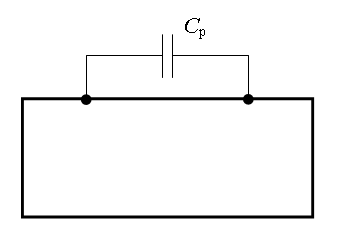
\includegraphics[width=6cm]{figures/fig1.png}%
 \caption{Tytuł rysunku, rozmiar 11 pkt, pojedyncza interlinia, akapit wyśrodkowany, bez wcięcia pierwszego wiersza. Na końcu tytułu rysunku/tabeli nie stawia się kropki [8]}%
 \label{Fig:schemat}%
\end{figure}

\begin{example}
[\ldots] Na rysunku \ref{Fig:wykres} pokazano przykładową zależność prądów pasmowych $i_\mathrm{ph}$ bezszczotkowego silnika prądu stałego z magnesami trwałymi w funkcji położenia wirnika $\theta$.
\end{example}

\begin{figure}[ht]
	\centering
	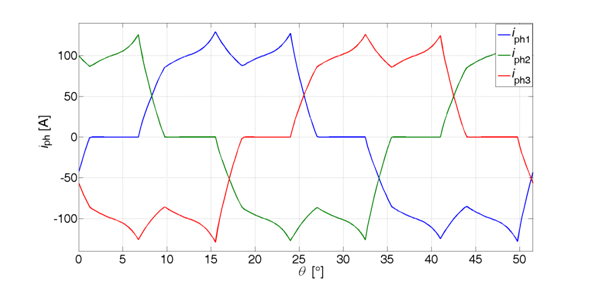
\includegraphics[width=12cm]{figures/fig2.png}
	\caption{Tytuł rysunku, rozmiar 11 pkt, pojedyncza interlinia, akapit wyśrodkowany, bez wcięcia pierwszego wiersza. Na końcu tytułu rysunku/tabeli nie stawia się kropki [8]}
\label{Fig:wykres}
\end{figure}


\begin{example}
[\ldots] oraz indukcyjności wzajemnej. W tabeli \ref{Tab:tabela} przedstawiono podstawowe parametry obwodu nieliniowego, zasilanego napięciem trójfazowym.
\end{example}

\begin{table}[ht]
\caption{Tytuł tabeli, rozmiar 11 pkt, pojedyncza interlinia, akapit wyrównany do lewej}
\centering		
	\begin{tabular}{|c|c|c|c|c|}	
		\hline
		$U$ [V] & $I$ [mA] & $R$, [k$\Omega$] & $L$ [mH] & $R/R_{20}$ \\
		\hline
		13,6 & 7,29 & 3,94 & 100 & 1,25 \\
		\hline
	\end{tabular}	
	
\label{Tab:tabela}
\end{table}	

\subsubsection{Wzory matematyczne}

Zmienne we wzorach pisze się czcionką pochyłą (styl edytora równań ,,Matematyka') natomiast symbole, niebędące zmiennymi, czcionką prostą (styl ,,Tekst'').
Rozmiary czcionek: normalny 12 punktów, indeks dolny/górny 9 pkt, indeks podrzędny 7 pkt, symbol 24 pkt, podsymbol 12 pkt Separatorem dziesiętnym w liczbach jest
przecinek, a nie kropka (dotyczy to również liczb pisanych w tekście akapitu). Poddaj się w tym zakresie \LaTeX{}owi - pisz wzór, a poprawnie się utworzy.


Pod wzorem należy zamieścić objaśnienia użytych symboli (chyba, że znajdują się w wykazie na początku pracy). Wzory umieszcza się wyśrodkowane i numeruje zgodnie
z kolejnością w danym rozdziale: (numer\_rozdziału.numer\_wzoru). Numery wzorów wyrównuje się do prawego marginesu. W akapicie poprzedzającym wzór musi znajdować się krótki opis, czego dotyczy dany wzór i – jeżeli potrzeba – odwołanie do literatury.

\begin{example}
[\ldots] wyznacza się, na podstawie wyrażenia (\ref{Eq:rownanie}). W nawiasach podano rozmiary czcionek używanych we wzorach
\end{example}

\begin{equation}
A(12)={\sum}(24)m_{s(9)}N^{k_{p(7)}}
\label{Eq:rownanie}
\end{equation}
gdzie: $m_s$ -- masa próbki, $N$ -- natężenie oświetlenia, $k_p$ -- wykładnik potęgi $(k_p=1,3-2,1)$.\\


\subsubsection{Listingi programów}

W pracy dyplomowej możesz umieszczać fragmenty programów. Pamiętaj, aby umieszczać krótkie, tylko najważniejsze fragmenty kodów źródłowych. Zawsze je komentuj w treści
pracy dyplomowej. Typowo w \LaTeX\ kody źródłowe umieszczane są w środowisku verbatim (\verb|\begin{verbatim}...\end{verbatim}|). Obecnie instnieje jednak bardziej nowoczesne i bardziej funkcjonalne środowisko \verb|lstlisting| (wymaga zainstalowanego w systemie pakietu \verb|listings|). Zwróć uwagę, że możesz kolorować składnię
automatycznie za pomocą parametru \verb|language|. W niniejszym dokumencie przedstawiono dwa przykłady listingów, Listing \ref{KodMatlab1} to przykład kodu źródłowego Matlaba, a poniżej Listing \ref{KodPerl1} dla Perl'a.\\
%\komentarz{

\begin{lstlisting}[language=Matlab,caption=Listing programu Matlab,label={KodMatlab1}]
i = 1
p = 3
for i = 1:10
    if i > 3
        i=i+p
    else 
        i=i+1
    end
end
\end{lstlisting}

\begin{lstlisting}[language=Perl,caption=Listing programu Perl,label={KodPerl1}]
  my $url ='http://pei.prz.edu.pl';
  use LWP::Simple;
  my $content = get $url;
  die "Couldn't get $url" unless defined $content;
  print $content;
  print "\n";
  print "Length " + length($content)
\end{lstlisting}

Z pewnością przeglądając źródło tego dokumentu zobaczysz, że kody źródłowe powinny mieć zdefiniowane parametry \verb|label|, aby łatwo w tekście do nich się odwoływać.
Numeracja linii jest w stylu domyślnie włączona (to przydatne, bo w treści pracy łatwo odwołać się dzięki temu do konkretnego wiersza w kodzie źródłowym), możesz je wyłączyć podając jako parametr \verb|numbers=none|. Więcej szczegółów możesz odnaleźć w sekcji \verb|\lstset| pliku arkusza styli. 
%}


\subsubsection{Numerowanie i punktowanie}

\begin{enumerate}[label=\arabic*), leftmargin=1.25cm]
	\item Pierwszy poziom (stosuje się numerowanie lub punktowanie). Formatowanie:
	akapit wyjustowany, wcięcie od lewej 0,75 cm, wysunięcie co 0,5 cm.
	\item Znakiem numerowania jest liczba (z kropką lub nawiasem).
		\begin{itemize}[label={--},labelsep=0.4cm,leftmargin=0.6cm]
			\item drugi poziom (stosuje się wyłącznie punktowanie). Formatowanie: akapit
			wyjustowany, wcięcie od lewej 1,25 cm, wysunięcie co 0,5 cm,
			\item znakiem punktowania jest łącznik lub mała litera alfabetu (z nawiasem). Nie
			zaleca się stosowania kropek, strzałek itp.,
			\item punktowane akapity rozpoczyna się minuskułą (małą literą), na końcu akapitu
			stawia się przecinek, ostatni punktowany akapit kończy się kropką.
		\end{itemize}
	\item Numerowane akapity rozpoczyna się majuskułą (wielką literą) i kończy kropką.
	\item Należy zwrócić uwagę, aby nie rozdzielać numerowania/punktowania pomiędzy
	kolejnymi stronami tekstu.
\end{enumerate}


\subsection{Wykaz literatury}

W wykazie literatury zamieszcza się wyłącznie pozycje, na które powołano się
w pracy. Kolejność numerów w wykazie – zgodna z kolejnością pojawiania się danej
pozycji w tekście.

Format akapitu: akapit wyjustowany, wysunięcie 0,75 cm. Prawidłowo opracowany
wykaz został zaprezentowany w niniejszym dokumencie w odpowiednim rozdziale, oznaczonym jako ,,Literatura''  (pozycja nr \cite{str} to zasoby internetowe,
\cite{Jakubczyk1997} – książka, \cite{Barski2011} – artykuł w czasopiśmie, \cite{dokum} – karta katalogowa).

\subsection{Wydruk pracy}

Przed wydrukiem należy usunąć ewentualne błędy literowe i sprawdzić prawidłową
interpunkcję.
Przykładowo, łącznik zapisuje się za pomocą krótkiego minusa (np.
badawczo-rozwojowy) natomiast myślnik -- stosowany w zdaniach wtrąconych -- zapisuje
się za pomocą długiej pauzy.
Dzielenie wyrazów według uznania autora (można podzielić
długie wyrazy, powodujące duże ,,rozstrzelenie'' tekstu w poprzedzającym wierszu.
Zaleca się usunięcie pojedynczych znaków na końcu wiersza przez zastosowanie w \LaTeX{} znaku tyldy w~tekście.
Dla przedrostka ,,mikro'' należy unikać stosowania litery ,,u'' czy ,,$\mu$'' zamiast ,,\microS''. 
Znak stopień otrzymuje poleceniem \kod{\symbol{36}\symbol{94}\symbol{92}circ\symbol{36}}.
W celu uniknięcia ,,rozstrzelenia'' liczb i ich jednostek zaleca się używanie ,,twardej'' spacji pomiędzy liczbą i jednostką (znak tyldy w \LaTeX{} ,,\kod{\symbol{126}}''.
Należy sprawdzić, czy tytuły
podrozdziałów/zakresów nie zostały jako pojedyncze wiersze na poprzedniej stronie oraz
czy rysunki/tabele i ich tytuły nie zostały rozdzielone pomiędzy kolejnymi stronami.

Pracę drukuje się dwustronnie. Zaleca się wydruk w kolorze. Przed wydrukiem
należy ponumerować strony (czcionka 10 pkt, dół strony, akapit wyśrodkowany).
Strony tytułowej oraz strony z podziękowaniem pozostawia się bez widocznego numeru strony.
Spis treści rozpoczyna się od strony numer 3 (lub 5, jeżeli zamieszczono podziękowania).


\section{Podsumowanie i wnioski końcowe}

1 $\div$ 3 stron merytorycznie podsumowanie najważniejszych elementów pracy oraz wnioski wynikające z osiągniętego celu pracy. Proponowane zalecenia i modyfikacje oraz rozwiązania będące wynikiem realizowanej pracy.

Ostatni akapit podsumowania musi zawierać wykaz własnej pracy dyplomanta i zaczynać się od sformułowania: ,,Autor za własny wkład pracy uważa: \ldots''.


\section*{Załączniki}
\addcontentsline{toc}{section}{Załączniki}

Według potrzeb zawarte i uporządkowane uzupełnienie pracy o dowolny materiał źródłowy (wydruk programu komputerowego, dokumentacja kons\-truk\-cyj\-no-\-tech\-no\-lo\-gicz\-na, konstrukcja modelu -- makiety -- urządzenia, instrukcja obsługi urządzenia lub stanowiska laboratoryjnego, zestawienie wyników pomiarów i obliczeń, informacyjne materiały katalogowe itp.).


\clearpage

\addcontentsline{toc}{section}{Literatura}

\begin{thebibliography}{4}
\bibitem{str} http://weii.portal.prz.edu.pl/pl/materialy-do-pobrania. Dostęp 5.01.2015.
\bibitem{Jakubczyk1997} Jakubczyk T., Klette A.: Pomiary w akustyce. WNT, Warszawa 1997.
\bibitem{Barski2011} Barski S.: Modele transmitancji. Elektronika praktyczna, nr 7/2011, str. 15-18.
\bibitem{dokum} Czujnik S200. Dokumentacja techniczno-ruchowa. Lumel, Zielona Góra, 2001.
\bibitem{Pawluk2001} Pawluk K.: Jak pisać teksty techniczne poprawnie, Wiadomości Elektrotechniczne, Nr 12, 2001, str. 513-515.
\end{thebibliography}

\clearpage

\makesummary

\end{document} 
